\chapter*{Conclusions and future works}
This thesis addressed the automatized visual analysis of peripheral blood cells images, with particular efforts on WBC analysis firstly and RBC, secondly. It has been focused on cells analysis and counting for diagnosing diseases using a microscope, a crucial step to confirm if and which illness is present. The main purpose has been the analysis of the outstanding issues in a CAD from digital microscopy images, particularly Acute Lymphoblastic Leukemia for WBCs and malaria for RBCs. It shows the studies addressed to some possible solutions for cells analysis and counting. Special efforts have been focused on strategies to represent with meaningful information the visual content of digital images. Indeed this issue is critical in artificial vision and becomes further challenging in medical imaging, considering that there is not a color standardization for the staining and acquisition of digital slides. There are several color differences or intensity variations between different slides, due to the quality of the biological sample and the sample preparation, such as the quantity of dye used during the staining procedure, or due to different acquisition systems and the image capturing parameters, such as the environment illumination. Furthermore, mainly in peripheral blood images, such variability may be present in the same slide, due to the presence of uneven lighting caused by the microscope light. Thus, by computing descriptors that ignore this variability, it is possible to extract from the images more general information that may be used by conventional learning models for distinguishing different biological concepts, avoiding any dependency on a specific dataset. 

Peripheral blood image analysis has been faced with special efforts towards the segmentation and the counting of both types of cells, either leukocytes and erythrocytes, proposing different segmentation algorithms able to isolate the cell of interest from images acquired in different illumination conditions and with different staining strategies.
The experimental results demonstrated that the final approach is very accurate and robust in relation to some traditional methods. It has been able to obtain an average accuracy of 100\% in WBC detection and 98 \%  in RBC detection. The 2\% difference is due to the fact that a lot of RBC tend to overlap other RBCs, so that it becomes quite tricky, even for human eye, discover their exact number. The results in this phase have also permitted to identify and count the WBCs correctly, that can be directly used to support some existing medical methods, like the WBCC. 
The identification of single WBCs is also essential for the diagnosis of leukemia, for which the cell components must be analyzed in detail, in order to find the morphological changes that can be observed in the cells affected by that disease.  Consequently, a further extension could be devoted to the realization of a complete cells classification system, able to distinguish among the several types of WBCs.

Moreover, the identification of RBCs has also been made in standard cell conditions, which is represented by the dataset in WBC analysis. For this reason, this work also contains a new public dataset specifically built and designed for malaria analysis purposes.

It is important to note that many of the proposed approaches could also be used in different medical imaging system and also for artificial vision system far from the medical field. It could be possible thanks to the generality of the proposed approaches, that is designed to overcome many different issues, such as the color differences, that make them independent from dataset and in some cases also from the problem itself.

Despite the good results obtained with both case studies, further improvements can be realized for peripheral blood image analysis. Many other phases can be integrated. 
In particular, a first improvement could arise from a detailed analysis of the WBCs in order to detect the type of disease that can affect a cell. 
Moreover, the realized system could also be extended to malaria parasite analysis by using the proposed dataset. Once single cells of each type have been detected and segmented, they can be analyzed in detail, to detect the presence of the parasite, like malaria parasite or to diagnose disease that can affect that particular cell type.   
It can even be extended to provide new measures, like the parasitemia percentage of an image.
These measures can be diagnostic by themselves, since that an overproduction or an underproduction is always a symptom of problems related to the health of the bone marrow. Adapting the system to bone marrow smear images analysis could be another exciting and useful task. Cells in bone marrow differ from peripheral blood cell images because there are only immature cells, so that shape and colors are not the same of peripheral blood cells either due to the absence of standard acquisition techniques or their characteristics. An example is shown underneath.

Finally, we should consider another important aspect which is arising a lot of importance in the community. Deep learning is increasingly used in computer vision and medical image analysis field. However, it is clear that applying deep learning algorithms to medical image analysis presents several unique challenges. The lack of large training data sets is often mentioned as an obstacle, especially in the case of microscopic image analysis. Although medical procedures nowadays tend to release a lot of images from medical procedures, one of the main challenge is also the acquisition of relevant annotations/labeling for these images.
Even when data is annotated by domain expert, label noise can be a significant limiting factor in developing algorithms, whereas in computer vision the noise in the labeling of images is typically relatively low. Training a deep learning system on such data requires careful consideration of how to deal with noise and uncertainty in the reference standard. One partial solution could be incorporating labeling uncertainty directly in the loss function, but this is still an open challenge.
In medical imaging often classification or segmentation is presented as a binary task: normal versus abnormal, object versus background. However, this is often a gross simplification as both classes can be highly heterogeneous. For example, in our case, the normal category consists of completely normal blood cells but also several categories of leukemia or parasites exist for the abnormal category. This often leads to systems that are extremely good at excluding the most common normal subclasses, but fail miserably on several rare ones. A straightforward solution would be to turn the deep learning system in a multi-class system by providing it with detailed annotations of all possible subclasses. From a certain point of view, this thesis also faced this issue at a first approximation. More efforts can be made in order to improve the solution. 


\begin{figure}[h]
	\centering
	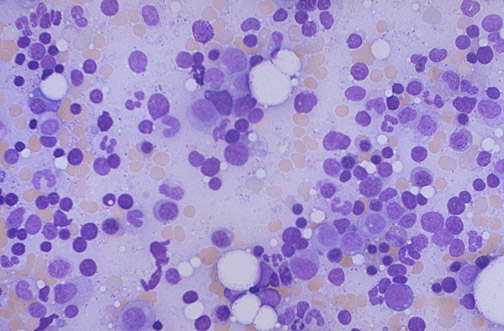
\includegraphics[width=0.5\textwidth]{images/bone_marrow}
	\caption[Bone marrow smear image.]{\label{fig:bone_marrow} Bone marrow smear image. Erythroid and granulocytic precursors are present. Courtesy of \cite{Med_Utah}}
\end{figure}